\chapter{Topic: Two dice sum}
{ }\hfill\textbf{Niveau:} Medium\\ \\
By rolling two dice, the sum of the scores on the two dice is an integer between  2 and 12. Here, we're going to see the different probabilities for each integer to appear and represent this with a graphical diagram.
\section{Simulating rolling one die.}
\noindent To simulate rolling a die, we're going to use the primitive \texttt{random}. Here's how it works:.\\ \\
\texttt{random 6} $\longrightarrow$ returns a randomly choosen integer  among 0, 1, 2, 3, 4, 5.\\
Hence, \texttt{(random 6)+1 } returns a randomly choosen integer from 1, 2, 3, 4, 5, 6. We need the parenthesis, otherwise, the \logo\ interpreter should understand \texttt{random 7}. To avoid parenthesis, we can write \texttt{1+random~6} too.\\ \\
We define the primitive called \texttt{die} which simulates rolling one die.
\begin{verbatim}
to die
   output 1+random 6
 end
\end{verbatim}
 \section{The program}
  We're going to use the multiturtle mode and the primitive \texttt{setturtle}. \texttt{setturtle} followed by an integer allows us to select the turtle whose identifier is the integer.\\ \\
  A good schema is better than a thousand explanations....
\begin{center}
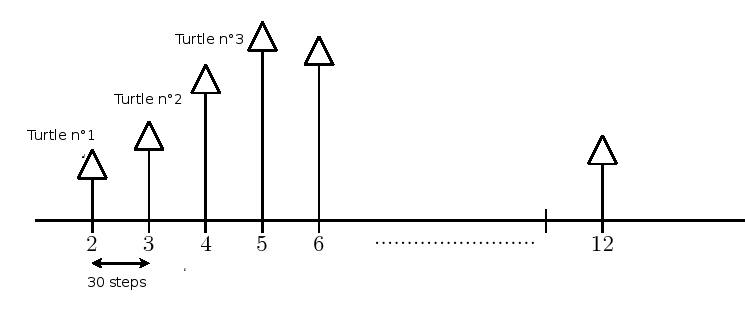
\includegraphics[scale=0.45]{pics/somme-des-schema.png}
\end{center}
\vspace{0.5cm}
Each turtle whose integer is from 2 o 12 will forward one step, when the corresponding dice sum appears. For example, if the two dice scores is 8, then turtle number 8 will forward one step. Between two turtle, there are 30 steps horizontally.\\ \\
We set all turtles using coordinates.
\begin{itemize}
 \item  The turtne n\degre2 has coordinates $(-150;0)$
 \item  The turtne n\degre3 has coordinates $(-120;0)$
 \item  The turtne n\degre4 has coordinates $(-90;0)$
 \item  The turtne n\degre5 has coordinates $(-60;0)$\\
\begin{minipage}{8 cm}
\begin{center}
 $\vdots$
\end{center}
\end{minipage}
\end{itemize}
\begin{verbatim}
 setturtle 2 setpos [-150 0]
 setturtle 3 setpos [-120 0]
 setturtle 4 setpos [-90 0]
 setturtle 5 setpos [-60 0]
 setturtle 6 setpos [-30 0]
.....
\end{verbatim}
Better than writing 11 times the same command line, we're going to use the primitive \texttt{for}. With this primitive, we can give a variable a sequence of values. Here, we want that the variable \texttt{:i} to have succesive values 2, 3, 4, ... , 12. We write:\\
\texttt{for [i 2 12] [ list of instructions]}\\ \\
To set up all the turtles we create the procedure \texttt{initialize}
\begin{verbatim}
to initialize
  cs ht pu
  for [i 2 12] [ 
      # Set up the turtle
      setturtle :i setpos list -150+(:i-2)*30 0
      # We write turtle number 15 steps under 
      pu bk 15 label :i fd 15 pd 
  ]
end
\end{verbatim}

You must understand the expression \texttt{-150+(:i-2)*30}. We're beginning from $-150$, and for each new turtle we add 30. (Test with the different values for \texttt{:i} if you're sceptic)\\ \\
Finally this is the program:
\begin{verbatim}
to die
   output 1+random 6
 end

to initialize
  cs ht pu
  for [i 2 12] [ 
      # Set up the turtle
      setturtle :i setpos list -150+(:i-2)*30 0
      # We write turtle number 15 steps under 
      pu bk 15 label :i fd 15 pd 
  ]
end

to go
initialize
# We make 1000 tries
repeat 1000 [
  make "sum die+die
  setturtle :sum fd 1
]
# We display frequencies
for [i 2 12] [
  setturtle :i
  # The Y-coordinates of each turle represents the number of times
  # a dice scores has appeared
  localmake "number last pos 
  pu fd 10 lt 90 fd 10 rt 90 pd label :number/1000*100
]
end
\end{verbatim}
Here is a more general program. We'll ask the user the number of dice he wants and the number of tries to make.
\begin{verbatim}

to initialize
  cs ht pu setturtlesmax :max+1
  for sentence list "i :min :max [ 
      # Set up the turtle
      setturtle :i setpos list -150+(:i-2)*30 0
      # We write turtle number 15 steps under 
      pu bk 15 label :i fd 15 pd 
  ]
end
to die
localmake "somme 0
repeat :dice [
   localmake "somme :somme+1 +random 6
 ]
output :somme
end

to go
read [Number of dice:] "dice
if not numberp :dice [print [Not a valid number!] stop]
globalmake "min :dice
globalmake "max 6*:dice
read [Number of tries to make: ] "tries
if not numberp :tries [print [labellength nombre rentré n'est pas valide!] stop]
initialize
# We make tries
repeat :tries [
  setturtle die forward 1
]
# Display frequencies
for sentence list "i :min :max [
  setturtle :i
  # Y-Axis coordinates represent the number of times a score has appeared
  localmake "effectif last position 
  # Round to 0.1
  penup forward 10 left 90 forward 10 right 90 pendown label (round :effectif/:tries*1000)/10
]
end


\end{verbatim}